%&LaTeX
\documentclass[11pt]{article}


% keep the following two lines; makes very nice pdf files when using ps2pdf
\usepackage[T1]{fontenc}
\usepackage{ae,aecompl}

\usepackage[normalem]{ulem}
\usepackage{fullpage}
\usepackage{setspace}
\usepackage{type1cm} % computer modern fonts
\usepackage{fancyhdr}
\usepackage{natbib}
%\usepackage[sort]{natbib}
%\usepackage{epsfig,psfrag,amsmath,amssymb,subfigure,setspace,rotating}
\usepackage{graphicx,psfrag,amsmath,amssymb,subfigure,setspace,rotating}

\usepackage{enumitem}

\usepackage[perpage,para,symbol]{footmisc}

\usepackage[usenames]{color}  % allows colored text

%\usepackage[sort]{natbib}
%\usepackage{epsfig,psfrag,amsmath,amssymb,subfigure}

% Mike's new commands \comm and \kill: uncomment if you want to use
\newcommand{\comm}[1]{\textcolor{blue}{\textit{#1}}}
\renewcommand{\kill}[1]{\textcolor{red}{\sout{#1}}}

\setlength{\parindent}{0.in}
\setlength{\parskip}{0.1in}

\newenvironment{itemize*}%
{\begin{itemize}[label=\textbullet,leftmargin=1pc,labelsep=*,noitemsep,
topsep=0.3pc,parsep=0.4pc]}
 {\end{itemize}}


%\pagestyle{fancy}
%\lhead{Wind-Turbine Structural Dynamics}
%\chead{}
%\rhead{2011 LDRD Proposal}




% \textheight=10.0in


\newcommand{\ie}{\textit{i.e.},~}
\newcommand{\eg}{\textit{e.g.},~}
\newcommand{\bs}{\boldsymbol}
\newcommand{\Ss}{\scriptscriptstyle}
\newcommand{\D}{\mathrm{d}}

\begin{document}  


\section*{Proposed geometric entities and data structures for code coupling
in FAST}

Michael A. Sprague \& John Michalakes, Draft, 7 December 2011

\section{Motivation, goals, notes}

\begin{itemize}

\item This document is towards defining an appropriate coupling framework
for FAST and FAST-related programs.  

\item A motivation is to provide consistent guidance to developers to
provide interface data in a standardized manner that simplifies coupling
with other components.

\item Any framework must general enough to explore/incorporate various
algorithmic coupling approaches.

\end{itemize}

\section{Geometric entities for coupling}

We assume that the ``physical'' interface of a component is either one of
the following or some combination:

\begin{enumerate} 
\item a point  (\eg  connection of a mooring line)

\item a line (may be curved) (\eg a beam representation of a blade)

\item a surface (\eg pressure distribution over a blade)

\item a volume (\eg OpenFOAM finite volume)

\end{enumerate}

These four geometric entities can be well described in a standard
isoparametric mapping, which is closely related to the finite-element
method; see Figs. 1-3.  

The elements and numbering schemes shown in Figs. 1-3 define unique
interpolation.  The inclusion of midside nodes allows for unique
representation of curved line/surface with quadratic polynomials.  The
elements shown in Figs. 1-3 are standard elements, and are available in most
meshing software.


\textbf{Remark:} Using a finite-element representation of component
interfaces has nothing to do with the discretization used by the underlying
components.

Interface elements:

Point: point

Line (Fig. 1): two-node (linear) or three-node (quadratic) line elements

Surface (Fig. 2): 3-node \& 6-node triangles elements; 4-node \& 8-node 
quadrilateral elements

Volume (Fig. 3): 8-node \& 20-node hexahedral elements;  
6-node \& 15-node wedge-elements;
4-node \& 10-node tetrahedron elements

\textbf{Remarks:} Figs. 1-3 show a standard numbering scheme. Linear-element 
numbering is a subset of the quadratic-element numbering shown.  For
example, a linear quadrilateral is defined just by the corner nodes, 1--4.

\section{Internal Representation data structures}
\label{sec:internal}

This section is intended to illustrate how components comprised of elements may be represented
at a low, essentially invisible level in the FAST coupling interface. The actual details of this
representation may differ from the description below, and will be hidden from the user 
within opaque objects accessed through 
Mesh Representation library routines, interfaces for which are proposed in 
Section \ref{sec:api}.

Here we assume we have a model where we know global position coordinates at
each "node" along with one or more number of degrees of freedom that are
known at each node.   In this description, we consider a single degree of
freedom, say displacement $u$.  Other degrees of freedom might by
temperature, rotation, local coordinates, etc.  Further, in addition to
scalar quantities, we could pass  vector, or tensor quantities.

\textbf{Approach:}\\
Assume that we have $N$ nodes on the boundary of the domain associated with
one code.  
Provide all boundary data as a $N$-dimensional real/double-precision arrays,
including global data positions and degrees of freedom (here $u$); 
\begin{verbatim}
integer N                    ! number of boundary nodes
double precision  xyz(N,3)   ! global xyz coordinates on bndry
double precision  u(N)       ! u response on bndry
\end{verbatim}

Create integer arrays that describe how the above boundary nodes are
connected, using elements described above:
\begin{verbatim}
integer Npoint               ! number of point elements
integer Nline2               ! number of 2-node line elements
integer Nline3               ! number of 3-node line elements
integer Ntri3                ! number of 3-node triangle elements
integer Ntri6                ! number of 6-node triangle elements
integer Nquad4               ! number of 4-node quadrilateral elements
integer Nquad8               ! number of 8-node quadrilateral elements
integer Ntet4                ! number of 4-node tet elements
integer Ntet10               ! number of 10-node tet elements
integer Nhex8                ! number of 8-node hex elements
integer Nhex10               ! number of 20-node hex elements
integer Nwedge6              ! number of 6-node wedge elements
integer Nwedge15             ! number of 15-node wedgeelements

integer element_point(Npoint)        ! point connectivity
integer element_line2(2,Nline2)      ! 2-node line connectivity
integer element_line3(3,Nline3)      ! 3-node line connectivity
integer element_line2(2,Ntri3)       ! 3-node triangle connectivity
integer element_line3(3,Ntri6)       ! 6-node triangle connectivity
integer element_quad4(4,Nquad4)      ! 4-node quad connectivity
integer element_quad8(8,Nquad8)      ! 8-node quad connectivity
integer element_tet4(4,Ntet4)        ! 3-node tet connectivity
integer element_tet10(10,Ntet10)     ! 10-node tet connectivity
integer element_hex8(8,Nhex8)        ! 8-node hex connectivity
integer element_hex20(20,Nhex20)     ! 20-node hex connectivity
integer element_wedge6(6,Nwedge6)    ! 6-node wedge connectivity
integer element_wedge15(15,Nwedge15) ! 15-node wedge connectivity

\end{verbatim}

With the above definition data can be uniquely interpolated from the nodal
values in $u$.

\textbf{Remark:} There is any number of ways that we could store and
transfer the above data.  The chosen form is verbose, but is clear.  We may
want to make it more succinct.  For example, the numbers of various elements
could be placed into a single integer array.  

%
%
%
%
%
%We wish to be able to transfer input-output properties across the coupled
%interface.  This is specific to the "self" domain.  For example, say we have
%a square surface defined by a single 4-node element.  The data required to
%build a coupling routine could be embodied as (\# denotes a comment line).
%Here we assume that output data is available at nodes, and the locations
%required for input data are defined in element-level natural coordinates.
%For example, for the following surface element, we want input forcing/data
%at Gauss points.
%
%\textbf{Remark:} The following is a ``text file'' realization of what could
%easily be a data stream transferred between programs to build up the
%coupling structure.  Following what is shown could be a list of all data
%available at each node, e.g. displacements, locations, etc.
%
%\clearpage
%\begin{verbatim}
%#--------------------------------------------------------------------
%#---------------- nodes  --------------------------------------------
%# number of nodes
%4
%# node number and locations:  num, x, y, z
%1 0. 0. 0.
%2 1. 0. 0.
%3 0. 1. 0.
%4 1. 1. 0.
%#--------------------------------------------------------------------
%#---------------- point elements ------------------------------------
%# number of point elements
%0
%# point-element definitions: number of nodes, n1, n2, ... 
%# number of input-points (None if no elements)
%# surface-element input-points (in element natural coordinates)
%#--------------------------------------------------------------------
%#---------------- line elements -------------------------------------
%# number of line elements
%0
%# line-element definitions: number of nodes, n1, n2, ... 
%# number of input-points (None if no elements)
%# surface-element input-points (in element natural coordinates)
%#--------------------------------------------------------------------
%#---------------- surface elements ----------------------------------
%# number of surface elements
%1
%# surface-element definitions: number of nodes, n1, n2, ... 
%4 1 2 4 3
%# number of input-points (none if no elements)
%4
%# surface-element input-points (in element natural coordinates)
%-0.577 -0.577
% 0.577 -0.577
%-0.577  0.577
% 0.577  0.577 
%#--------------------------------------------------------------------
%#---------------- volume elements -----------------------------------
%# number of volume elements
%0
%# volume-element definitions: number of nodes, n1, n2, ... 
%# number of input-points (None if no elements)
%# surface-element input-points (in element natural coordinates)
%
%\end{verbatim}
%
%
%
%
%
\begin{figure}[h!p]
\centering
     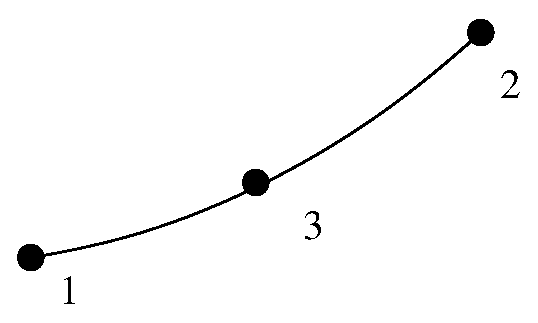
\includegraphics[width=1.8in]{figs/line3.xfig.eps}
     \caption{Element connectivities for line
     elements. Numbering for linear (1--2) and quadratic (1--3) elements are
     shown.}
\end{figure}

\begin{figure}[h!p]
\centering
    \subfigure[]{
     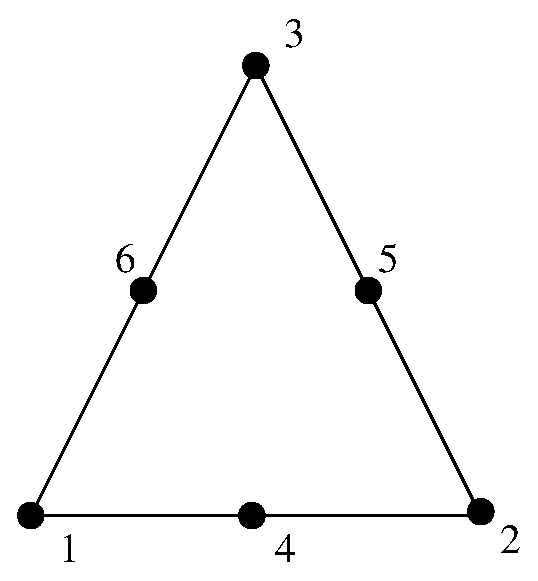
\includegraphics[width=1.8in]{figs/tri6.xfig.eps}} \hspace{0.4in}
     \subfigure[]{
     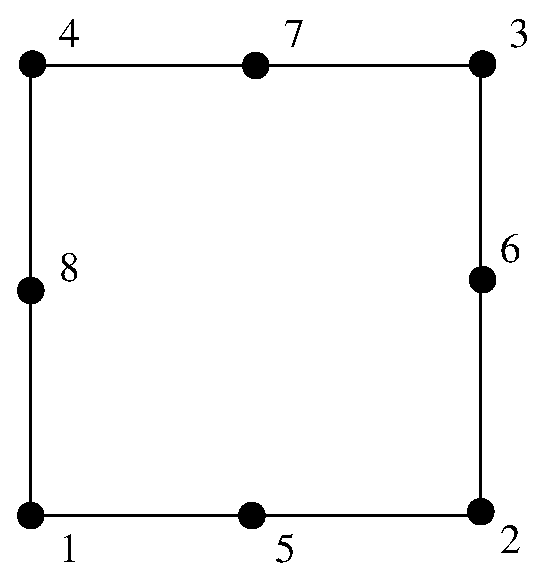
\includegraphics[width=1.8in]{figs/square8.xfig.eps}} \hspace{0.4in}
     \caption{Element connectivities for triangle and square surface
     elements. Numbering for linear and quadratic (serendipity) elements are
     shown.}
\end{figure}


\begin{figure}[h!p]
\centering
    \subfigure[]{
     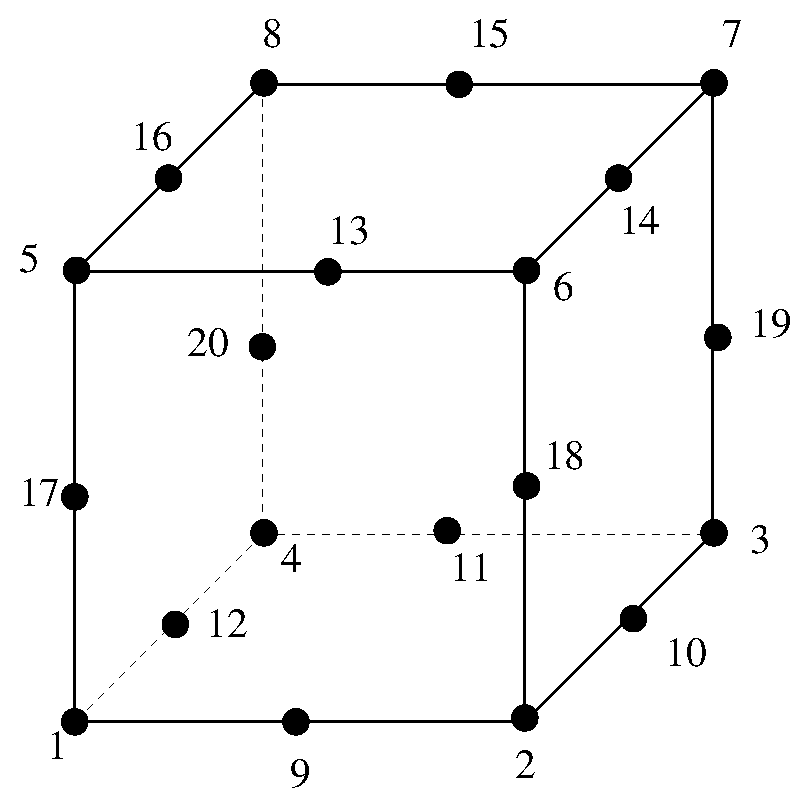
\includegraphics[width=2.5in]{figs/hex.xfig.eps}} \hspace{0.4in}
     \subfigure[]{
     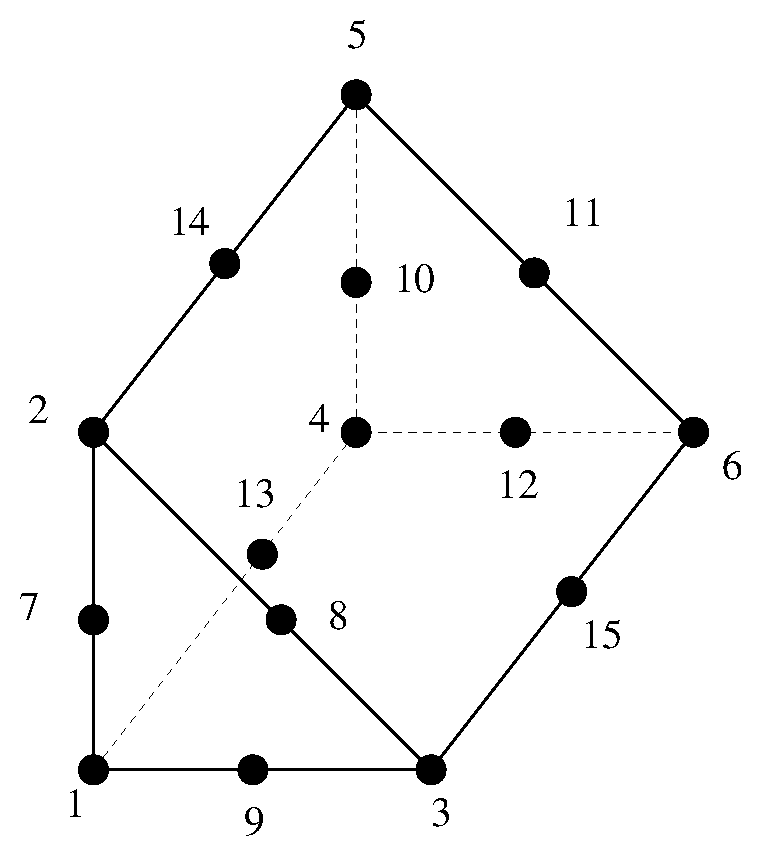
\includegraphics[width=2.5in]{figs/wedge.xfig.eps}} \hspace{0.4in}
     \subfigure[]{
     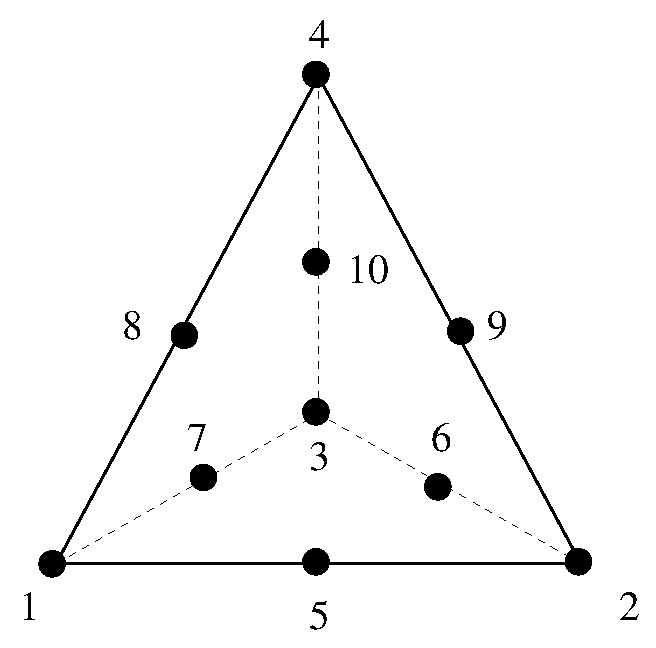
\includegraphics[width=2.5in]{figs/tet.xfig.eps}} \hspace{0.4in}
     \caption{Element connectivities for hexagonal, wedge, and tet
     elements. Numbering for linear and quadratic (serendipity) elements are
     shown.}
\end{figure}


\section{FAST Interface API}
\label{sec:api}
This section desribes a proposal for a user-visible Application Program Interface (API) for the
FAST inter-module mesh representation (FIMMR) described in Section \ref{sec:internal}. The proposal
is not a complete API specification yet, nor is the illustrative code working examples.  The examples
are in Fortran but a fully specified API will also contain C/C++ interfaces as well.

The data objects for the proposed interface are State Vectors of type REAL(ReKi) (following the
FAST real type convention) and integer Mesh Vectors, one per structural component being passed 
between FAST modules. There are two forms of State Vector, one for Markers and one for Loads.  Each
element of a Marker vector contains:

\begin{verbatim}
   REAL(ReKi)                 :: Position(3)
   REAL(ReKi)                 :: Orientation(3,3)     ! Direction Cosine Matrix (DCM)
   REAL(ReKi)                 :: TranslationVel(3)
   REAL(ReKi)                 :: RotationVel(3)
\end{verbatim}

Each element of a Load vector contains:

\begin{verbatim}
   REAL(ReKi)                 :: Force(3)
   REAL(ReKi)                 :: Moment(3)
\end{verbatim}

These are not accessed directly; rather, the elements are set or retrieved using routines in the 
FIMMR API.  The information shown in Section \ref{sec:internal} that represents the various aspects of
a mesh being passed through the coupling interface is packed into the State and Component vectors, which
can then be passed between different modules as one-dimensional arrays of simple data types even if the modules
are written in different languages.  This avoids avoids the troublesome issue of passing derived data types between
C and Fortran.  The Component Vectors, which are integer arrays, contain the mesh layout and topologies as well
as indices for each point of an element into the real typed State Vectors that contain the values for the 
different properties such as Position, Orientation, Force, Momentum, etc.  Users of the interface are specifically
advised against assuming anything about the layout of the State and Component vectors; nor would it be useful
or advisable for users to access the contents of the vectors directly.  One reason for this is that the 
actual layout is apt to change over time.  Relying on the FIMMR interface routines will ensure that 
changes or extensions to the underlying data representation will have no effect on existing
interface-compatible code.

Some of the envisioned interface routines for accessing or storing elements in State Vectors passed through
the FIMMR interface are listed below and described in the subsections that follow in this Section.
A complete listing of a sample routine showing calls to the FIMMR API routines is listed
in Section \ref{sec:listing}.
The MeshRet set of FIMMR routines below are fuctions used to retrieve elements 
from a State Vector (provided as one argument) 
using the indexing and other layout information encoded into the Component Vector for a particular 
structural componet; for example, a turbine blade.  Another set, the MeshPut subroutines, are
used to store elements back into a vector.  The last routine sketched below is a utility that allows 
copying between two sets of State/Component vectors to store or retrieve a local copy of the mesh
within a routine.


\subsection{MeshRetMarkerOrient}
Return a vector of Orientations (DIMENSION(3,3))from a marker state vector for a given component.
Optional argument IElement is the index of the element to return, 1 if omitted.
Optional argument N is the number of orientations to return, 1 if omitted.
\begin{verbatim}
FUNCTION MeshRetMarkerOrient ( 
                               MarkerStateVec
                              ,ComponentVec 
                             [,I ,N ]
                             [,Ierr]
                             )
   REAL(ReKi), INTENT(IN   ) :: MarkerStateVec
   INTEGER,    INTENT(IN   ) :: ComponentVec
   INTEGER,    INTENT(IN   ), OPTIONAL :: I
   INTEGER,    INTENT(IN   ), OPTIONAL :: N
   INTEGER,    INTENT(  OUT), OPTIONAL :: Ierr 		! non-zero if error
      ! Returns:
   REAL(ReKi), DIMENSION(3,3,N) :: MeshRetMarkerOrient
\end{verbatim}

\subsection{MeshRetMarkerRotVel}
Return a vector of Rotation Velocities (DIMENSION(3)) from a marker state vector for a given component.
Optional argument IElement is the index of the element to return, 1 if omitted.
Optional argument N is the number of orientations to return, 1 if omitted.
\begin{verbatim}
FUNCTION MeshRetMarkerRotVel ( 
                               MarkerStateVec
                              ,ComponentVec 
                             [,IElement ,N ]
                             [,Ierr]
                             )
   REAL(ReKi), INTENT(IN   ) :: MarkerStateVec(:)
   INTEGER,    INTENT(IN   ) :: ComponentVec(:)
   INTEGER,    INTENT(IN   ), OPTIONAL :: IElement
   INTEGER,    INTENT(IN   ), OPTIONAL :: N
   INTEGER,    INTENT(  OUT), OPTIONAL :: Ierr 		! non-zero if error
      ! Returns:
   REAL(ReKi), DIMENSION(3,N) :: MeshRetMarkerRotVel
\end{verbatim}

\subsection{MeshRetMarkerPosition}
Return a vector of Positions (DIMENSION(3)) from a marker state vector for a given component.
Optional argument IElement is the index of the element to return, 1 if omitted.
Optional argument N is the number of orientations to return, 1 if omitted.
\begin{verbatim}
FUNCTION MeshRetMarkerPosition ( MarkerStateVec
                                ,ComponentVec 
                               [,IElement ,N ]
                               [,Ierr]
                               )
   REAL(ReKi), INTENT(IN   ) :: MarkerStateVec(:)
   INTEGER,    INTENT(IN   ) :: ComponentVec(:)
   INTEGER,    INTENT(IN   ), OPTIONAL :: IElement
   INTEGER,    INTENT(IN   ), OPTIONAL :: N
   INTEGER,    INTENT(  OUT), OPTIONAL :: Ierr 		! non-zero if error
      ! Returns:
   REAL(ReKi), DIMENSION(3,N) :: MeshRetMarkerPosition
\end{verbatim}

\subsection{MeshRetLoadForce}
Return a vector of Forces (DIMENSION(3)) from a load state vector for a given component.
Optional argument IElement is the index of the element to return, 1 if omitted.
Optional argument N is the number of orientations to return, 1 if omitted.
\begin{verbatim}
FUNCTION MeshRetLoadForce (      LoadStateVec
                                ,ComponentVec 
                               [,IElement ,N ]
                               [,Ierr]
                               )
   REAL(ReKi), INTENT(IN   ) :: LoadStateVec(:)
   INTEGER,    INTENT(IN   ) :: ComponentVec(:)
   INTEGER,    INTENT(IN   ), OPTIONAL :: IElement
   INTEGER,    INTENT(IN   ), OPTIONAL :: N
   INTEGER,    INTENT(  OUT), OPTIONAL :: Ierr 		! non-zero if error
      ! Returns:
   REAL(ReKi), DIMENSION(3,N) :: MeshRetLoadForce
\end{verbatim}

\subsection{MeshRetLoadMoment}
Return a vector of Moments (DIMENSION(3)) from a load state vector for a given component.
Optional argument IElement is the index of the element to return, 1 if omitted.
Optional argument N is the number of orientations to return, 1 if omitted.
\begin{verbatim}
FUNCTION MeshRetLoadMoment (      LoadStateVec
                                ,ComponentVec 
                               [,IElement ,N ]
                               [,Ierr]
                               )
   REAL(ReKi), INTENT(IN   ) :: LoadStateVec(:)
   INTEGER,    INTENT(IN   ) :: ComponentVec(:)
   INTEGER,    INTENT(IN   ), OPTIONAL :: IElement
   INTEGER,    INTENT(IN   ), OPTIONAL :: N
   INTEGER,    INTENT(  OUT), OPTIONAL :: Ierr 		! non-zero if error
      ! Returns:
   REAL(ReKi), DIMENSION(3,N) :: MeshRetLoadMoment
\end{verbatim}

\subsection{MeshPutMarkerOrient}
Set a vector of Orientations (DIMENSION(3,3)) in a marker state vector for a given component.
Argument IElement is the index of the element to be set.
Optional argument N is the number of orientations to return, 1 if omitted.
\begin{verbatim}
SUBROUTINE MeshPutMarkerOrient ( 
                               MarkerStateVec
                              ,ComponentVec 
                              ,Orientations
                              ,IElement
                             [,N ]
                             [,Ierr]
                             )
   REAL(ReKi), INTENT(IN   ) :: MarkerStateVec(:)
   INTEGER,    INTENT(IN   ) :: ComponentVec(:)
   REAL(ReKi), INTENT(IN   ) :: Orientations(3,3,:)
   INTEGER,    INTENT(IN   ) :: IElement
   INTEGER,    INTENT(IN   ), OPTIONAL :: N
   INTEGER,    INTENT(  OUT), OPTIONAL :: Ierr 		! non-zero if error
\end{verbatim}

\subsection{MeshPutMarkerRotVel}
Set a vector of Rotation Velocities (DIMENSION(3)) in a marker state vector for a given component.
Argument IElement is the index of the element to be set.
Optional argument N is the number of orientations to return, 1 if omitted.
\begin{verbatim}
SUBROUTINE MeshPutMarkerRotVel ( 
                               MarkerStateVec
                              ,ComponentVec 
                              ,RotationVelocities
                              ,IElement
                             [,N ]
                             [,Ierr]
                             )
   REAL(ReKi), INTENT(IN   ) :: MarkerStateVec(:)
   INTEGER,    INTENT(IN   ) :: ComponentVec(:)
   REAL(ReKi), INTENT(IN   ) :: RotationVelocities(3,:)
   INTEGER,    INTENT(IN   ) :: IElement
   INTEGER,    INTENT(IN   ), OPTIONAL :: N
   INTEGER,    INTENT(  OUT), OPTIONAL :: Ierr 		! non-zero if error
\end{verbatim}

\subsection{MeshPutMarkerPosition}
Set a vector of Positions (DIMENSION(3)) in a marker state vector for a given component.
Argument IElement is the index of the element to be set.
Optional argument N is the number of orientations to return, 1 if omitted.
\begin{verbatim}
SUBROUTINE MeshPutMarkerPosition ( 
                               MarkerStateVec
                              ,ComponentVec 
                              ,Positions
                              ,IElement
                             [,N ]
                             [,Ierr]
                             )
   REAL(ReKi), INTENT(IN   ) :: MarkerStateVec(:)
   INTEGER,    INTENT(IN   ) :: ComponentVec(:)
   REAL(ReKi), INTENT(IN   ) :: Positions(3,:)
   INTEGER,    INTENT(IN   ) :: IElement
   INTEGER,    INTENT(IN   ), OPTIONAL :: N
   INTEGER,    INTENT(  OUT), OPTIONAL :: Ierr 		! non-zero if error
\end{verbatim}

\subsection{MeshPutLoadForce}
Set a vector of Forces (DIMENSION(3)) in a load state vector for a given component.
Argument IElement is the index of the element to be set.
Optional argument N is the number of orientations to return, 1 if omitted.
\begin{verbatim}
SUBROUTINE MeshPutLoadForce ( 
                               MarkerStateVec
                              ,ComponentVec 
                              ,Forces
                              ,IElement
                             [,N ]
                             [,Ierr]
                             )
   REAL(ReKi), INTENT(IN   ) :: MarkerStateVec(:)
   INTEGER,    INTENT(IN   ) :: ComponentVec(:)
   REAL(ReKi), INTENT(IN   ) :: Forces(3,:)
   INTEGER,    INTENT(IN   ) :: IElement
   INTEGER,    INTENT(IN   ), OPTIONAL :: N
   INTEGER,    INTENT(  OUT), OPTIONAL :: Ierr 		! non-zero if error
\end{verbatim}

\subsection{MeshPutLoadMoment}
Set a vector of Moments (DIMENSION(3)) in a load state vector for a given component.
Argument IElement is the index of the element to be set.
Optional argument N is the number of orientations to return, 1 if omitted.
\begin{verbatim}
SUBROUTINE MeshPutLoadMoment ( 
                               MarkerStateVec
                              ,ComponentVec 
                              ,Moments
                              ,IElement
                             [,N ]
                             [,Ierr]
                             )
   REAL(ReKi), INTENT(IN   ) :: MarkerStateVec(:)
   INTEGER,    INTENT(IN   ) :: ComponentVec(:)
   REAL(ReKi), INTENT(IN   ) :: Moment(3,:)
   INTEGER,    INTENT(IN   ) :: IElement
   INTEGER,    INTENT(IN   ), OPTIONAL :: N
   INTEGER,    INTENT(  OUT), OPTIONAL :: Ierr 		! non-zero if error
\end{verbatim}

\subsection{MeshCopyComponentLoads}
Copy a vector of loads from one load state vector to another.
\begin{verbatim}
SUBROUTINE MeshCopyComponentLoads( SrcLoadStateVec
                                  ,SrcComponentVec
                                  ,DestLoadStateVec
                                  ,DestComponentVec
                                 [,Ierr]
                                 )
   REAL(ReKi), INTENT(IN   ) :: SrcLoadStateVec(:)
   INTEGER,    INTENT(IN   ) :: SrcComponentVec(:)
   REAL(ReKi), INTENT(  OUT) :: DestLoadStateVec(:)
   INTEGER,    INTENT(  OUT) :: DestComponentVec(:)
   INTEGER,    INTENT(  OUT), OPTIONAL :: Ierr
\end{verbatim}


\begin{verbatim}
\end{verbatim}


\section{Example: AD\_CalcualateLoads}
\label{sec:listing}

This example listing below is from the AeroDyn module of FAST and is intended to show
the definition of a FAST module that uses the FIMMR interface and API routines.
Original
lines of executable code are retained as comments beginning with '!jm'.  This is a non-working
example, intended to illustrate the use of the FIMMR API when it is fully implemented.
Some of the
source lines have been reformatted to fit on a page.  

{\scriptsize
\begin{verbatim}
  1  !===========================================================================
  2  FUNCTION AD_CalculateLoads( CurrentTime, TurbineIndex                      &
  3                             ,InMarkers, Configuration                       &
  4                             ,OutLoads                                       &
  5                             ,Blades, Hub, RotorFurl, Nacelle, Tower, Tail   &
  6                            )
  7  ! Main AeroDyn procedure, calcs loads of the elements given by InMarkers
  8  !---------------------------------------------------------------------------
  9     USE                           AeroTime 
 10     USE                           AeroSubs
 11     USE                           domain_mod
 12  
 13        ! Passed parameters
 14  
 15     REAL( ReKi ),           INTENT(IN   ) :: CurrentTime
 16     INTEGER,                INTENT(IN   ) :: TurbineIndex       ! Turbine index 
 17                                                                 ! (used to manage internal state in 
 18                                                                 !  multi-turbine code)
 19        ! Markers associated with mesh points
 20     REAL( ReKi ),           INTENT(IN   ) :: InMarkers(:)       ! these are opaque to be
 21     REAL( ReKi ),           INTENT(IN   ) :: ConfigMarkers(:)   ! accessed only through FIMMR API
 22        ! Loads associated with mesh points
 23     REAL( ReKi ),           INTENT(  OUT) :: OutLoads(:)
 24        ! Component meshes
 25     INTEGER,                INTENT(IN   ) :: Blades(:,:)        
 26     INTEGER,                INTENT(IN   ) :: Hub(:)
 27     INTEGER,                INTENT(IN   ) :: RotorFurl(:)
 28     INTEGER,                INTENT(IN   ) :: Nacelle(:)
 29     INTEGER,                INTENT(IN   ) :: Tower(:)
 30  
 31        ! Function definition
 32  
 33        ! Local variables
 34  
 35     INTEGER    :: NB  ! number of blades
 36     REAL(ReKi), PARAMETER               :: OnePlusEpsilon = 1 + EPSILON(CurrentTime)
 37     INTEGER,                INTENT(OUT) :: ErrStat           ! Determines if an error encountered
 38     REAL(ReKi)                 :: VNElement
 39     REAL(ReKi)                 :: VelNormalToRotor2
 40     REAL(ReKi)                 :: VNWind
 41     REAL(ReKi)                 :: VTTotal
 42     REAL(ReKi)                 :: DFN
 43     REAL(ReKi)                 :: DFT
 44     REAL(ReKi)                 :: PMA
 45     REAL(ReKi)                 :: SPitch                     ! sine of PitNow
 46     REAL(ReKi)                 :: CPitch                     ! cosine of PitNow
 47  
 48     REAL(ReKi)                 :: AvgVelNacelleRotorFurlYaw
 49     REAL(ReKi)                 :: AvgVelTowerBaseNacelleYaw
 50     REAL(ReKi)                 :: AvgVelTowerBaseYaw
 51     REAL(ReKi)                 :: AzimuthAngle
 52     REAL(ReKi)                 :: rNacelleHub   (2)
 53     REAL(ReKi)                 :: rLocal
 54     REAL(ReKi)                 :: rRotorFurlHub (2)
 55     REAL(ReKi)                 :: rTowerBaseHub (2)
 56     
 57     REAL(ReKi)                 :: tmpVector     (3)
 58     REAL(ReKi)                 :: tmpVector1    (3)
 59     REAL(ReKi)                 :: tmpVector2    (3)
 60     REAL(ReKi)                 :: tmpVector3    (3)
 61     REAL(ReKi)                 :: VelocityVec   (3)
 62     REAL(ReKi)                 :: HubOrient       (3,3)
 63     REAL(ReKi)                 :: RotorFurlOrient (3,3)
 64  
 65     INTEGER                    :: IBlade
 66     INTEGER                    :: IElement
 67  
 68     INTEGER                    :: i   ! misc counting variable
 69  
 70     REAL( ReKi ),           INTENT(IN   ) :: LocLoads(:)
 71     INTEGER,                INTENT(IN   ) :: LocBlades(:,:)
 72     INTEGER,                INTENT(IN   ) :: LocHub(:)
 73     INTEGER,                INTENT(IN   ) :: LocRotorFurl(:)
 74     INTEGER,                INTENT(IN   ) :: LocNacelle(:)
 75     INTEGER,                INTENT(IN   ) :: LocTower(:)
 76  
 77     !!!=== SL
 78     include 'NWTC_ptr_dec.inc'
 79     include 'aerotime_ptr_dec.inc'
 80     include 'airfoil_ptr_dec.inc'
 81     include 'blade_ptr_dec.inc'
 82     include 'element_ptr_dec.inc'
 83     include 'eloutparams_ptr_dec.inc'
 84     include 'inducedvel_ptr_dec.inc'
 85     include 'rotor_ptr_dec.inc'
 86     include 'switch_ptr_dec.inc'
 87  
 88     include 'NWTC_ptr_set.inc'
 89     include 'aerotime_ptr_set.inc'
 90     include 'airfoil_ptr_set.inc'
 91     include 'blade_ptr_set.inc'
 92     include 'element_ptr_set.inc'
 93     include 'eloutparams_ptr_set.inc'
 94     include 'inducedvel_ptr_set.inc'
 95     include 'rotor_ptr_set.inc'
 96     include 'switch_ptr_set.inc'
 97     !!!=== end SL
 98  
 99        ! Executable statements
100  
101     !---------------------------------------------------------------------------
102     ! Check that the module has been initialized.
103     !---------------------------------------------------------------------------
104     IF ( .NOT. Initialized ) THEN
105        CALL WrScr( 'AeroDyn must be initialized before trying to calculate aerodynamic loads.' )
106        ErrStat = 1
107        RETURN
108     ELSE
109        ErrStat = 0
110     END IF
111  
112     !---------------------------------------------------------------------------
113     ! Determine if loads should be recalculated or just returned
114     !---------------------------------------------------------------------------
115        ! NOTE: CurrentTime is scaled by OnePlusEps to ensure that loads are calculated at every
116     !       time step when DTAero = DT, even in the presence of numerical precision errors.
117  
118     NB = SIZE(Blades,2)
119  
120     IF ( NoLoadsCalculated .OR. ( CurrentTime*OnePlusEpsilon - OldTime ) >= DTAERO )  THEN
121           ! It's time to update the aero forces
122  
123           ! First we reset the DTAERO parameters for next time
124        DT      = CurrentTime - OldTime     ! DT = 0 on first step, but the subroutines 
125                                            ! that use DT check for NoLoadsCalculated (or time > 0)
126        OldTime = CurrentTime
127  
128     ELSE IF ( .NOT. CurrentADOptions%LinearizeFlag ) THEN
129  
130           ! Return the previously-calculated loads
131       
132        i = TurbineIndex
133        DO IBlade = 1,NB
134          CALL MeshCopyComponentLoads( LocBlades(:,IBlade,i), LocLoads(:,i), Blades(Iblade), OutLoads )
135        ENDDO
136        CALL MeshCopyComponentLoads( LocHub(:,i),       LocLoads(:,i), Hub,       OutLoads )
137        CALL MeshCopyComponentLoads( LocRotorFurl(:,i), LocLoads(:,i), RotorFurl, OutLoads )
138        CALL MeshCopyComponentLoads( LocNacelle(:,i),   LocLoads(:,i), Nacelle,   OutLoads )
139        CALL MeshCopyComponentLoads( LocTower(:,i),     LocLoads(:,i), LocTower,  OutLoads )
140  
141        RETURN
142  
143     ENDIF
144  
145     HubOrientation            = MeshRetMarkerOrient  ( ConfigMarkers, Hub )
146     HubRotationVel            = MeshRetMarkerRotVel  ( ConfigMarkers, Hub )
147     HubPosition               = MeshRetMarkerPosition( ConfigMarkers, Hub )
148     RotorFurlOrientation      = MeshRetMarkerOrient  ( ConfigMarkers, RotorFurl )
149     RotorFurlRotationVelocity = MeshRetMarkerRotVel  ( ConfigMarkers, RotorFurl )
150     RotorFurlPosition         = MeshRetMarkerPosition( ConfigMarkers, RotorFurl )
151     NacelleOrientation        = MeshRetMarkerOrient  ( ConfigMarkers, Nacelle )
152     NacelleRotationVel        = MeshRetMarkerRotVel  ( ConfigMarkers, Nacelle )
153     NacellePosition           = MeshRetMarkerPosition( ConfigMarkers, Nacelle )
154     TowerOrientation          = MeshRetMarkerOrient  ( ConfigMarkers, Tower )
155     TowerRotationVel          = MeshRetMarkerRotVel  ( ConfigMarkers, Tower )
156     TowerPosition             = MeshRetMarkerPosition( ConfigMarkers, Tower )
157  
158     !---------------------------------------------------------------------------
159     ! Calculate the forces and moments for the blade: 
160     !                            SUBROUTINE AeroFrcIntrface( FirstLoop, JElemt, DFN, DFT, PMA )
161     !---------------------------------------------------------------------------
162     Time      = CurrentTime
163  
164        ! calculate rotor speed
165        ! note: Subtracting the RotorFurl rotational velocity for REVS is needed to get the
166        ! same answers as before v13.00.00. RotorFurl shouldn't be needed.
167  
168  !jm   REVS = ABS( DOT_PRODUCT( TurbineComponents%Hub%RotationVel(:) - &
169  !jm                                          TurbineComponents%RotorFurl%RotationVel(:), &
170  !jm                                 TurbineComponents%Hub%Orientation(1,:) ) )
171  
172  ! interface call functions
173     REVS      = ABS( DOT_PRODUCT( HubRotationVel(:) - RotorFurlRotationVel(:), &
174                                   HubOrient(1,:)
175  
176        ! calculate yaw angle
177        ! note: YawAng should use the Hub instead of the RotorFurl, but it is calculated this way to
178        ! get the same answers as previous version.
179  !jm   YawAng    = ATAN2( -1.*TurbineComponents%RotorFurl%Orientation(1,2), &
180  !jm                                     TurbineComponents%RotorFurl%Orientation(1,1) ) 
181     YawAng    = ATAN2( -1.*RotorFurlOrientation(1,2), RotorFurlOrientation(1,1) )
182     SYaw      = SIN( YawAng )
183     CYaw      = COS( YawAng )
184  
185        ! tilt angle
186        ! note: tilt angle should use the Hub instead of RotorFurl, but it needs hub to get the same
187        ! answers as the version before v13.00.00
188        
189  !jm   Tilt      = ATAN2( TurbineComponents%RotorFurl%Orientation(1,3), &
190  !jm                SQRT( TurbineComponents%RotorFurl%Orientation(1,1)**2 + &
191  !jm                      TurbineComponents%RotorFurl%Orientation(1,2)**2 ) )
192  
193     Tilt      = ATAN2( RotorFurlOrientation(1,3), &
194                  SQRT( RotorFurlOrientation(1,1)**2 + &
195                        RotorFurlOrientation(1,2)**2 ) )
196  
197     CTilt     = COS( Tilt )
198     STilt     = SIN( Tilt )
199        
200        ! HubVDue2Yaw - yaw velocity due solely to yaw
201        
202  !jm  AvgVelNacelleRotorFurlYaw = TurbineComponents%RotorFurl%RotationVel(3) - &
203  !jm                                                TurbineComponents%Nacelle%RotationVel(3)
204  !jm  AvgVelTowerBaseNacelleYaw = TurbineComponents%Nacelle%RotationVel(3)   - &
205  !jm                                                TurbineComponents%Tower%RotationVel(3)
206  !jm  AvgVelTowerBaseYaw        = TurbineComponents%Tower%RotationVel(3)    
207    AvgVelNacelleRotorFurlYaw = RotorFurlRotationVel(3) - NacelleRotationVel(3)
208    AvgVelTowerBaseNacelleYaw = NacelleRotationVel(3)   - TowerRotationVel(3)
209    AvgVelTowerBaseYaw        = TowerRotationVel(3)    
210        
211  !jm   rRotorFurlHub(1:2)        = TurbineComponents%Hub%Position(1:2) - &
212  !jm                                                TurbineComponents%RotorFurl%Position(1:2)
213  !jm   rNacelleHub(1:2)          = TurbineComponents%Hub%Position(1:2) - &
214  !jm                                                TurbineComponents%Nacelle%Position(1:2)
215  !jm   rTowerBaseHub(1:2)        = TurbineComponents%Hub%Position(1:2) - &
216  !jm                                                TurbineComponents%Tower%Position(1:2)
217     rRotorFurlHub(1:2)        = HubPosition(1:2) - RotorFurlPosition(1:2)
218     rNacelleHub(1:2)          = HubPosition(1:2) - NacellePosition(1:2)
219     rTowerBaseHub(1:2)        = HubPosition(1:2) - TowerPosition(1:2)
220  
221    YawVel =   ( AvgVelNacelleRotorFurlYaw * rRotorFurlHub(2) &
222                      + AvgVelTowerBaseNacelleYaw * rNacelleHub(2) &
223                      + AvgVelTowerBaseYaw * rTowerBaseHub(2) ) * SYaw &
224             - ( AvgVelNacelleRotorFurlYaw * rRotorFurlHub(1) &
225                      + AvgVelTowerBaseNacelleYaw * rNacelleHub(1) &
226                      + AvgVelTowerBaseYaw * rTowerBaseHub(1) ) * CYaw
227    
228     !...........................................................................
229     ! start of NewTime routine
230     !...........................................................................
231  
232     AvgInfl = SumInfl * 2.0 / (R*R*NB)        ! Compute average inflow from the previous time step
233     SumInfl = 0.0                             ! reset to sum for the current time step
234  
235     CALL DiskVel()                            ! Get a sort of "Average velocity" - 
236                                               !    sets a bunch of stored variables...
237  
238     IF ( DStall ) CALL BedUpdate()            ! update the old values to hold "current" values 
239                                               !    from last time step
240  
241     ! Enter the dynamic inflow routines here
242     IF ( Wake )  CALL Inflow()
243  
244     !...........................................................................
245     ! end of NewTime routine
246     !...........................................................................
247  
248  
249     DO IBlade = 1,NB
250     
251           ! calculate the azimuth angle ( we add pi because AeroDyn defines 0 as pointing downward)
252           ! note: the equation below should use TurbineComponents%Blade markers, but this is used to get the 
253           ! same answers as the previous version (before v13.00.00)                          
254           
255  !jm AzimuthAngle = ATAN2( -1.*DOT_PRODUCT( TurbineComponents%Hub%Orientation(3,:),         & 
256  !jm                                        TurbineComponents%RotorFurl%Orientation(2,:) ), &
257  !jm                           DOT_PRODUCT( TurbineComponents%Hub%Orientation(3,:),         &
258  !jm                                        TurbineComponents%RotorFurl%Orientation(3,:) )  ) &
259  !jm                                                               + pi + (IBlade - 1)*TwoPiNB
260        AzimuthAngle = ATAN2( -1.*DOT_PRODUCT( HubOrientation(3,:),         & 
261                                               RotorFurlOrientation(2,:) ), &
262                                  DOT_PRODUCT( HubOrientation(3,:),         &
263                                               RotorFurlOrientation(3,:) )  ) + pi + (IBlade - 1)*TwoPiNB
264  
265        BladeOrientation          = MeshRetMarkerOrient   ( ConfigMarkers, Blade(IBlade) )
266        BladeRotationVel          = MeshRetMarkerRotVel   ( ConfigMarkers, Blade(IBlade) )
267        BladePosition             = MeshRetMarkerPosition ( ConfigMarkers, Blade(IBlade) )
268  
269        DO IElement = 1,NElm
270  
271           BEOrientation    = MeshGetMarkerOrient  ( InputMarkers, Blade(IBlade), IElement )
272           BEPosition       = MeshGetMarkerPosition( InputMarkers, Blade(IBlade), IElement )
273           BEVelocity       = MeshGetMarkerVelocity( InputMarkers, Blade(IBlade), IElement )
274           BETranslationVel = MeshGetMarkerTransVel( InputMarkers, Blade(IBlade), IElement )
275              
276              ! calculate element pitch
277                                              
278  !jm         PitNow    = -1.*ATAN2( -1.*DOT_PRODUCT( TurbineComponents%Blade(IBlade)%Orientation(1,:),    &
279  !jm                                                 InputMarkers%Blade(IElement,IBlade)%Orientation(2,:) ) , &
280  !jm                                    DOT_PRODUCT( TurbineComponents%Blade(IBlade)%Orientation(1,:),    &
281  !jm                                                 InputMarkers%Blade(IElement,IBlade)%Orientation(1,:) )   )
282  
283           PitNow    = -1.*ATAN2( -1.*DOT_PRODUCT( BladeOrientation(1,:),    &
284                                                   BEOrientation(2,:) ) , &
285                                      DOT_PRODUCT( BladeOrientation(1,:),    &
286                                                   BEOrientation(1,:) )   )
287                      
288           SPitch    = SIN( PitNow )
289           CPitch    = COS( PitNow )
290  
291           
292              ! calculate distance between hub and element
293              
294  !jm         tmpVector = InputMarkers%Blade(IElement,IBlade)%Position(:) - TurbineComponents%Hub%Position(:)
295  !jm         rLocal = SQRT(   DOT_PRODUCT( tmpVector, TurbineComponents%Hub%Orientation(2,:) )**2  &
296  !jm                        + DOT_PRODUCT( tmpVector, TurbineComponents%Hub%Orientation(3,:) )**2  )
297           tmpVector = BEPosition(:) - HubPosition(:)
298           rLocal = SQRT(   DOT_PRODUCT( tmpVector, HubOrientation(2,:) )**2  &
299                          + DOT_PRODUCT( tmpVector, HubOrientation(3,:) )**2  )
300  
301  !jm If bjj doesn't know I'm sure I don't.... :)
302  !jm            ! determine if MulTabLoc should be set.  
303  !jm            ! bjj: I have no idea how this is really (supposed to be) used!!! .... 
304  !jm            
305  !jm         IF ( CurrentADOptions%SetMulTabLoc(IElement,IBlade)  ) THEN
306  !jm            MulTabLoc = CurrentADOptions%MulTabLoc(IElement,IBlade)
307  !jm         END IF
308           
309  
310           !...........................................................................
311           ! Get wind velocity components; calculate velocity normal to the rotor squared
312           ! Save variables for printing in a file later;
313           !...........................................................................
314  !jm  VelocityVec(:)    = AD_WindVelocityWithDisturbance( InputMarkers%Blade(IElement,IBlade)%Position(:) )
315           VelocityVec(:)    = AD_WindVelocityWithDisturbance( BEPosition(:) )
316           VelNormalToRotor2 = ( VelocityVec(3) * STilt + (VelocityVec(1) * CYaw &
317                                                - VelocityVec(2) * SYaw) * CTilt )**2
318  
319  
320           !---------------------------------------------------------------------------
321           ! reproduce GetVNVT routine:
322           !---------------------------------------------------------------------------
323  !jm         tmpVector =  -1.*SPitch*InputMarkers%Blade(IElement,IBlade)%Orientation(1,:) &
324  !jm                       + CPitch*InputMarkers%Blade(IElement,IBlade)%Orientation(2,:)
325  !jm         VTTotal   =     DOT_PRODUCT( tmpVector, VelocityVec &
326  !jm                           - InputMarkers%Blade(IElement,IBlade)%TranslationVel  )
327  !jm         tmpVector =     CPitch*InputMarkers%Blade(IElement,IBlade)%Orientation(1,:) &
328  !jm                                 + SPitch*InputMarkers%Blade(IElement,IBlade)%Orientation(2,:)
329  !jm         VNElement = -1.*DOT_PRODUCT( tmpVector, InputMarkers%Blade(IElement,IBlade)%TranslationVel )
330           tmpVector =  -1.*SPitch*BEOrientation(1,:) &
331                         + CPitch*BEOrientation(2,:)
332           VTTotal   =     DOT_PRODUCT( tmpVector, VelocityVec - BETranslationVel
333  
334           tmpVector =     CPitch*BEOrientation(1,:) &
335                                   + SPitch*BEOrientation(2,:)
336           VNWind    =     DOT_PRODUCT( tmpVector, VelocityVec )
337           VNElement = -1.*DOT_PRODUCT( tmpVector, BETranslationVel )
338  
339           !--------------------------------------------------------------------------
340           ! Get blade element forces and induced velocity
341           !--------------------------------------------------------------------------
342           CALL ELEMFRC( AzimuthAngle, rLocal, IElement, IBlade, VelNormalToRotor2, VTTotal, VNWind, &
343                         VNElement, DFN, DFT, PMA, NoLoadsCalculated )  
344  
345           !-------------------------------------------------------------------------------------------
346           ! Set up dynamic inflow parameters
347           !-------------------------------------------------------------------------------------------
348           IF ( DynInfl .OR. DynInit ) THEN
349              CALL GetRM (rLocal, DFN, DFT, AzimuthAngle, IElement, IBlade)
350           ENDIF
351  
352  !jm         ADCurrentLoads%Blade(IElement,IBlade)%Force(1)  = ( DFN*CPitch + DFT*SPitch ) / DR(IElement)
353  !jm         ADCurrentLoads%Blade(IElement,IBlade)%Force(2)  = ( DFN*SPitch - DFT*CPitch ) / DR(IElement)
354  !jm         ADCurrentLoads%Blade(IElement,IBlade)%Force(3)  = 0.0
355           tmpVector(1) = ( DFN*CPitch + DFT*SPitch ) / DR(IElement)
356           tmpVector(2) = ( DFN*SPitch - DFT*CPitch ) / DR(IElement)
357           tmpVector(3) = 0.0
358           CALL MeshPutLoadForce( LocLoads(:,TurbineIndex), LocBlades(:,Iblade,TurbineIndex), tmpVector, IElement )
359  
360  !jm         ADCurrentLoads%Blade(IElement,IBlade)%Moment(1) = 0.0
361  !jm         ADCurrentLoads%Blade(IElement,IBlade)%Moment(2) = 0.0
362  !jm         ADCurrentLoads%Blade(IElement,IBlade)%Moment(3) = PMA / DR(IElement)
363           tmpVector(1) = 0.0
364           tmpVector(2) = 0.0
365           tmpVector(3) = PMA / DR(IElement)
366           CALL MeshPutLoadMoment( LocLoads(:,TurbineIndex), LocBlades(:,Iblade,TurbineIndex), tmpVector, IElement )
367  
368              ! save velocities for output, if requested
369  
370           IF ( WndElPrList(IElement) > 0 ) THEN
371              SaveVX( WndElPrList(IElement), IBlade ) = VelocityVec(1)
372              SaveVY( WndElPrList(IElement), IBlade ) = VelocityVec(2)
373              SaveVZ( WndElPrList(IElement), IBlade ) = VelocityVec(3)
374           ENDIF
375           
376  
377        END DO !IElement
378  
379        IF ( IBlade == 1 .AND. ElemPrn ) THEN
380           VXSAV  = VelocityVec(1)
381           VYSAV  = VelocityVec(2)
382           VZSAV  = VelocityVec(3)
383        ENDIF
384  
385  
386     END DO !IBlade
387  
388     NoLoadsCalculated = .FALSE.
389     
390  !jm   AD_CalculateLoads = ADCurrentLoads
391  
392     i = TurbineIndex
393     DO IBlade = 1,NB
394       CALL MeshCopyComponentLoads( LocBlades(:,IBlade,i), LocLoads(:,i), &
395                                    Blades(Iblade),    OutLoads )  ! interface call
396     ENDDO
397     CALL MeshCopyComponentLoads( LocHub(:,i),       LocLoads(:,i), Hub,       OutLoads )
398     CALL MeshCopyComponentLoads( LocRotorFurl(:,i), LocLoads(:,i), RotorFurl, OutLoads )
399     CALL MeshCopyComponentLoads( LocNacelle(:,i),   LocLoads(:,i), Nacelle,   OutLoads )
400     CALL MeshCopyComponentLoads( LocTower(:,i),     LocLoads(:,i), LocTower,  OutLoads )
401  
402  END FUNCTION  AD_CalculateLoads
\end{verbatim}
}


%\bibliography{ref_template}
%\bibliographystyle{jfm}
%\bibliographystyle{chicago}
%\bibliographystyle{plain}

\end{document}  

